%% EduLogGen -- SoftwareX Original Software Publication (revised).
%% Structure of the SoftwareX OSP template (elsarticle class): code metadata,
%% 1 Motivation and significance, 2 Software description, 3 Illustrative
%% examples, 4 Impact, 5 Conclusions. Supplementary material: supplementary.tex.
\documentclass[preprint,12pt]{elsarticle}

\usepackage{amssymb}
\usepackage{booktabs}
\usepackage{graphicx}
\usepackage{hyperref}
\usepackage{listings}
\usepackage{orcidlink}
\usepackage{xcolor}

\lstset{
  basicstyle=\ttfamily\footnotesize,
  columns=fullflexible,
  keepspaces=true,
  breaklines=true,
  frame=single,
  framerule=0.3pt,
  commentstyle=\color{gray},
}

\journal{SoftwareX}

\begin{document}

\begin{frontmatter}

\title{EduLogGen: A Python package for generating and validating synthetic educational interaction logs}

\author[a]{Anis Bey\,\orcidlink{0000-0001-9410-0851}\corref{cor1}}
\cortext[cor1]{Corresponding author.}
\ead{beyanisse@gmail.com}
\address[a]{Higher School of Management Sciences, Annaba, Algeria}

\begin{abstract}
Interaction logs from learning platforms underpin learning analytics, but
they are personal data that are difficult to share, so methods are often
evaluated on a single private dataset and rarely against a known ground
truth. EduLogGen is an open-source Python package that ingests real logs with
pseudonymisation, fits interpretable Markov and semi-Markov generators,
produces seeded synthetic logs, validates them against real data with
fidelity metrics and privacy diagnostics, and benchmarks generators on
held-out learners. An experimental layer adds known ground truth: labelled
anomalies, controlled manipulations, and behavioural profiles. We evaluate
it on two public datasets: daily activity of 10{,}143 learners aggregated
into weekly sequences (OULAD), and fine-grained, timestamped app clickstreams
(EdNet). Markov generators reduced the bigram error of an order-blind
baseline by two thirds on OULAD and by about 90\% on EdNet, approaching but not
reaching the difference between two real learner samples; only the
semi-Markov and an optional GRU network generator reproduced inter-event
timing, and the untuned GRU was less faithful to event sequences than the
Markov models. Synthetic data were no closer to the training learners than
unseen real learners were, and
injecting anomalies into synthetic instead of real sessions overstated
detector performance on EdNet.
\end{abstract}

\begin{keyword}
learning analytics \sep educational data mining \sep synthetic data \sep
interaction logs \sep privacy \sep benchmarking
\end{keyword}

\end{frontmatter}

%% ---------------------------------------------------------------------------
\section*{Code metadata}
\noindent
\begin{small}
\begin{tabular}{p{0.06\linewidth}p{0.40\linewidth}p{0.46\linewidth}}
\toprule
Nr. & Code metadata description & Metadata \\
\midrule
C1 & Current code version & v1.5.0 \\
C2 & Permanent link to code/repository used for this code version & \url{https://github.com/anisbey1/EduLogGen/tree/v1.5.0} \\
C3 & Permanent link to Reproducible Capsule & \url{https://doi.org/10.5281/zenodo.23281595} \\
C4 & Legal Code License & MIT License \\
C5 & Code versioning system used & git \\
C6 & Software code languages, tools, and services used & Python; GitHub Actions; PyPI \\
C7 & Compilation requirements, operating environments \& dependencies & Python $\geq$ 3.11 (Linux, macOS, Windows); PyYAML; optional pyarrow, matplotlib, PyTorch (GRU generator); \texttt{pip install eduloggen} \\
C8 & If available, link to developer documentation/manual & \url{https://anisbey1.github.io/EduLogGen/} \\
C9 & Support email for questions & beyanisse@gmail.com \\
\bottomrule
\end{tabular}
\end{small}

%% ---------------------------------------------------------------------------
\section{Motivation and significance}

Interaction logs from learning management systems are the raw material of
learning analytics and educational data mining~\cite{romero2020edm}. They are
also personal data: sharing them across institutions, attaching them to
papers, or using them in teaching is restricted by privacy law and
institutional policy~\cite{drachsler2016delicate}. Many methods are therefore
evaluated on a single private dataset, results are hard to reproduce, and
tasks such as anomaly detection or learner clustering are rarely tested
against a known ground truth.

Synthetic data are a common answer~\cite{jordon2022synthetic}, and Berg et
al.\ argued for a reference synthetic data generator for learning
analytics~\cite{berg2016reference}. Existing tools cover only parts of this
need. Tabular synthesisers such as the Synthetic Data Vault~\cite{patki2016sdv}
and synthpop~\cite{nowok2016synthpop} model records, not ordered events
nested in sessions, learners, and courses. Process-mining
simulators~\cite{vanderaalst2016process} generate event logs from
hand-specified process models rather than learning behaviour from data, and
neither kind validates the output against held-out real learners or reports
disclosure risk. Synthetic data are not private by
construction~\cite{stadler2022groundhog}, so fidelity and memorisation must
be measured, yet researchers who need synthetic logs typically write one-off
scripts that do neither.

EduLogGen makes this workflow explicit, measurable, and reproducible. It
ingests real logs through a declarative mapping with pseudonymisation;
sessionises and analyses them; fits interpretable sequence generators;
generates seeded synthetic corpora; validates them against real data; and
benchmarks generators on held-out learners under versioned protocols. An
experimental layer generates data with \emph{known} ground truth (labelled
anomalies, deliberate manipulations, behavioural profiles) so that detection
and clustering methods can be scored against it.

%% ---------------------------------------------------------------------------
\section{Software description}

\subsection{Software architecture}

EduLogGen is a pure-Python, fully typed package with one required dependency
(PyYAML), organised in layers whose import rules are enforced by the test
suite (Fig.~\ref{fig:architecture}). Immutable data models (events, sessions,
datasets, models, annotations) underlie a pipeline of ingestion, analysis,
generators, validation, and benchmarking. The experimental layer is built on
top of the generators rather than inside them, and an evaluation module
scores methods against its ground truth. Users work through a Python API or a
command-line interface; readers, generators, metrics, and anomaly types can
be added as plugins.

Every random step derives its seed from one user seed, artifacts record
content fingerprints of their inputs, models are stored as JSON rather than
executable pickles, and outputs are written atomically, so a result can be
traced to its data, parameters, and seed and regenerated exactly with the
same package version.

\begin{figure}[t]
\centering
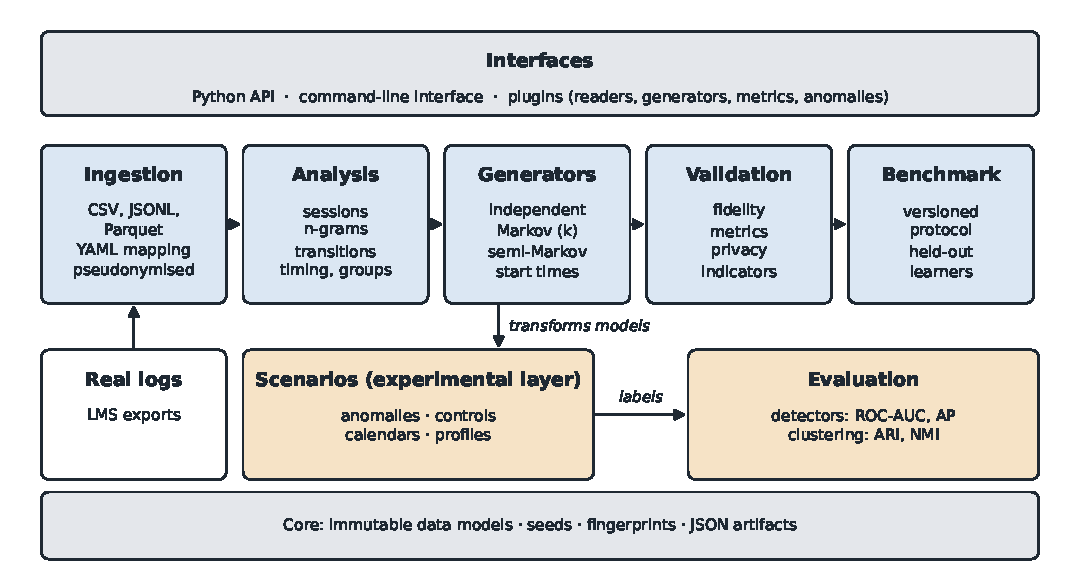
\includegraphics[width=\linewidth]{fig_architecture.pdf}
\caption{Architecture of EduLogGen. The main pipeline (blue) turns real logs
into validated and benchmarked synthetic corpora; the experimental layer
(orange) produces data with ground-truth labels and scores methods against
them.}
\label{fig:architecture}
\end{figure}

\subsection{Software functionalities}

\paragraph{Ingestion and sessionisation} A YAML mapping assigns source columns
to canonical fields (learner, timestamp, activity, event type, course, score,
success, duration), with optional salted hashing of identifiers and a data
quality report that contains no data values. Sessions come from explicit
identifiers, an idle timeout, or both.

\paragraph{Analysis} Event and activity mixes, $n$-grams, transitions,
session lengths and durations, time per activity, navigation graphs, temporal
patterns, and the same statistics per course, week, cohort, or metadata
field.

\paragraph{Generators} \texttt{independent} draws events from their overall
frequencies, ignoring order. \texttt{markov} draws the next event from a
first- or higher-order transition model with back-off, and the gap to the
next event from one distribution shared by all events. \texttt{semi\_markov}
uses the same transitions but draws each gap from the distribution of gaps
observed after the \emph{current} event type (empirical by default), so time
spent depends on the activity but not on the next one~\cite{yu2010hsmm}.
Gaps are measured within sessions only (zero gaps become 1~ms); gaps between
sessions, session lengths, sessions per learner, and start times are modelled
separately. The optional \texttt{gru} generator (\texttt{pip install
"eduloggen[neural]"}, PyTorch) is a recurrent network over the whole session
history: at each step it predicts the next event type and the time spent
after the current event, as a choice among quantile bins of the training
gaps from which an observed gap is then drawn, so discrete gaps such as whole
days are reproduced exactly. Its training (Adam, early stopping on a
validation split, sessions truncated to 256 events) is seeded and
deterministic on CPU, and its weights are stored inside the JSON model. All
generators share the models of session lengths, learners, and start times,
and generated identifiers are re-mapped so that no source identifier is
reproduced.

\paragraph{Validation} Real and synthetic corpora are compared with marginal
(event-type total variation distance, TVD; activity Jensen--Shannon
divergence, JSD), structural (session-length Kolmogorov--Smirnov, KS),
temporal (inter-event time KS), sequential (bigram TVD, transition JSD), and
navigation metrics (overlap of the ten most frequent paths). Privacy
diagnostics work on sessions as token sequences: the share of synthetic
sessions of at least three events identical to a real session, the share of
once-seen real trigrams reproduced, and edit distances to the nearest real
session. Reports state that these diagnostics estimate memorisation risk and
are not privacy guarantees.

\paragraph{Benchmarking} The versioned protocol \texttt{session\_fidelity\_v1}
splits learners 70/30 into training and holdout sets, fits each generator on
the training learners, generates three seeded samples of the holdout's size,
and compares each with the holdout. As a reference, it compares the
training with the holdout learners once, which shows how much two samples of
real learners differ.

\paragraph{Experimental layer} (i) Anomaly injection: five types (event
frequency, abnormal timing, unexpected transition, repetition, inactivity),
labelled as invalid workflow or unusual but valid behaviour and stored apart
from the events; injected sessions are disjoint, and an evaluator reports
ROC-AUC, average precision, and recall per type. Anomalies describe data
patterns and are never equated with misconduct. (ii) Controls re-weight
event types, scale time spent, fix session lengths or sessions per learner,
and apply course calendars with deadline surges, each verified by a
manipulation check against an uncontrolled baseline. These are controlled
capabilities; the case studies below do not validate calendar fidelity.
(iii) Behavioural profiles are learned by seeded
$k$-means++~\cite{arthur2007kmeanspp} on training learners only, imported, or
defined by hand; profile mixtures record each synthetic learner's profile,
and \texttt{evaluate\_clustering} reports the adjusted Rand index
(ARI)~\cite{hubert1985ari}, normalised mutual information (NMI), and purity.

\paragraph{Quality assurance} 1{,}024 automated tests (99\% line and branch
coverage) and strict static typing run in continuous integration on Python
3.11--3.13, together with an end-to-end pipeline and a documentation build;
tagged releases are published to PyPI and archived on Zenodo.

\subsection{Sample code snippets}

A complete workflow on the command line:
\begin{lstlisting}[language=bash]
eduloggen ingest --input events.csv --mapping map.yaml \
    --output corpus/
eduloggen sessionize --input corpus/ --output sessions/
eduloggen fit --input sessions/ --generator semi_markov \
    --output model/
eduloggen generate --model model/ --n-sessions 5000 \
    --seed 7 --output synthetic/
eduloggen validate --real sessions/ --synthetic synthetic/ \
    --output report/
eduloggen benchmark --input sessions/ --output benchmark/
\end{lstlisting}
The same in Python, followed by a profile-recovery experiment (the built-in
synthetic demo course stands in for real data):
\begin{lstlisting}[language=Python]
import eduloggen as elg
from eduloggen.benchmark import split_by_learner

data = elg.sessionize(elg.demo_dataset(200, seed=1))
train, holdout = split_by_learner(data, 0.3, seed=0)

model = elg.fit_generator("semi_markov", train)
synthetic = elg.generate(model, n_sessions=holdout.n_sessions,
                         seed=7)
print(elg.validate(holdout, synthetic).to_markdown())

profiles = elg.fit_profiles(train, n_profiles=3, seed=0)
mix = elg.generate_profiles(profiles, 2000, seed=1)
found = elg.fit_profiles(mix.dataset, n_profiles=3, seed=0)
labels = found.assign(mix.dataset)
print(elg.evaluate_clustering(mix.annotations, labels).ari)
\end{lstlisting}

%% ---------------------------------------------------------------------------
\section{Illustrative examples}

\subsection{Data}
\textbf{OULAD} (coarse-grained)~\cite{kuzilek2017oulad}: seven modules of
the 2014J presentation, 10{,}143 learners. OULAD records clicks per learner,
resource, and \emph{day} only, so we defined an event as an active
learner-day, typed by its most-clicked activity type, and a session as a
learner's module week. This is a benchmark of \emph{aggregated} weekly
activity: sequences have at most seven events, within-day order and
secondary activities are lost, and gaps are whole days.
\textbf{EdNet-KT4} (fine-grained)~\cite{choi2020ednet}: millisecond-timestamped
actions of a random sample of 2{,}000 students of a mobile learning app
(entering items, answering, erasing choices, submitting, playing and pausing
audio or video), typed as action plus item kind (17 event types) and
sessionised with a 30-minute idle timeout: 967{,}968 events in 10{,}580
sessions (median 49 events, 29\% with 100 or more, maximum 1{,}575). Scripts in \texttt{studies/} reproduce all results with
seed~0; per-module and per-seed results are in the supplementary material.

\subsection{Fidelity}
Table~\ref{tab:fidelity} and Fig.~\ref{fig:fidelity} report the benchmark.
All generators reproduced event-type frequencies and session-length
distributions with small discrepancies (TVD and KS at most 0.031 on OULAD and
0.086 on EdNet, against real-versus-real values of 0.020--0.022 and
0.039--0.084). Markov-based models
substantially improved sequential fidelity over the independent baseline
(bigram TVD 0.073--0.079 against 0.220 on OULAD; 0.059--0.063 against 0.655
on EdNet), although their bigram discrepancies remained above the
real-versus-real reference (0.038 and 0.052): about twice the reference on
the short OULAD weeks and 1.1--1.2 times on EdNet. The semi-Markov generator
additionally reproduced the inter-event gap distribution closely (KS 0.013
against 0.281 on OULAD; 0.028 against 0.507 on EdNet). The second-order model
did not improve on the first-order one. The GRU, used with its default
hyperparameters and without tuning, reproduced timing nearly as well as the
semi-Markov generator (KS 0.017 and 0.032) but was less faithful to event
sequences than the Markov models (bigram TVD 0.098 and 0.094; event-type TVD
0.047 and 0.054): a more flexible model does not guarantee higher fidelity,
which is why generators are compared on held-out learners.

\begin{table}[t]
\centering
\caption{Fidelity on held-out learners (mean $\pm$ SD: over modules for
OULAD, over three seeds for EdNet). ``Real vs real'' compares training with
holdout learners once per dataset; $\downarrow$ lower and $\uparrow$ higher is
better. TVD: total variation distance; JSD: Jensen--Shannon divergence; KS:
Kolmogorov--Smirnov statistic.}
\label{tab:fidelity}
\resizebox{\linewidth}{!}{\begin{tabular}{l r r r r r r }
\toprule
Metric & Real vs real & Independent & Markov-1 & Markov-2 & Semi-Markov & GRU \\
\midrule
\multicolumn{7}{l}{\textit{OULAD (7 modules)}} \\
Event-type TVD $\downarrow$ & 0.022 & 0.021 $\pm$ 0.004 & 0.028 $\pm$ 0.005 & 0.031 $\pm$ 0.011 & 0.027 $\pm$ 0.009 & 0.047 $\pm$ 0.014 \\
Bigram TVD $\downarrow$ & 0.038 & 0.220 $\pm$ 0.022 & 0.074 $\pm$ 0.015 & 0.079 $\pm$ 0.016 & 0.073 $\pm$ 0.011 & 0.098 $\pm$ 0.022 \\
Transition JSD $\downarrow$ & 0.002 & 0.049 $\pm$ 0.010 & 0.003 $\pm$ 0.002 & 0.003 $\pm$ 0.002 & 0.003 $\pm$ 0.001 & 0.005 $\pm$ 0.002 \\
Session-length KS $\downarrow$ & 0.020 & 0.023 $\pm$ 0.017 & 0.020 $\pm$ 0.014 & 0.020 $\pm$ 0.014 & 0.021 $\pm$ 0.017 & 0.022 $\pm$ 0.014 \\
Inter-event time KS $\downarrow$ & 0.010 & 0.281 $\pm$ 0.049 & 0.281 $\pm$ 0.049 & 0.281 $\pm$ 0.049 & 0.013 $\pm$ 0.011 & 0.017 $\pm$ 0.009 \\
Top-10 path overlap $\uparrow$ & 0.900 & 0.700 $\pm$ 0.115 & 0.833 $\pm$ 0.077 & 0.814 $\pm$ 0.112 & 0.838 $\pm$ 0.078 & 0.819 $\pm$ 0.121 \\
\midrule
\multicolumn{7}{l}{\textit{EdNet-KT4}} \\
Event-type TVD $\downarrow$ & 0.039 & 0.039 $\pm$ 0.000 & 0.047 $\pm$ 0.002 & 0.045 $\pm$ 0.002 & 0.048 $\pm$ 0.002 & 0.054 $\pm$ 0.005 \\
Bigram TVD $\downarrow$ & 0.052 & 0.655 $\pm$ 0.001 & 0.061 $\pm$ 0.002 & 0.059 $\pm$ 0.002 & 0.063 $\pm$ 0.002 & 0.094 $\pm$ 0.006 \\
Transition JSD $\downarrow$ & 0.004 & 0.488 $\pm$ 0.001 & 0.004 $\pm$ 0.000 & 0.004 $\pm$ 0.000 & 0.004 $\pm$ 0.000 & 0.009 $\pm$ 0.001 \\
Session-length KS $\downarrow$ & 0.084 & 0.079 $\pm$ 0.004 & 0.085 $\pm$ 0.003 & 0.085 $\pm$ 0.003 & 0.086 $\pm$ 0.003 & 0.089 $\pm$ 0.014 \\
Inter-event time KS $\downarrow$ & 0.019 & 0.507 $\pm$ 0.000 & 0.507 $\pm$ 0.000 & 0.507 $\pm$ 0.000 & 0.028 $\pm$ 0.000 & 0.032 $\pm$ 0.000 \\
Top-10 path overlap $\uparrow$ & 1.000 & 0.100 $\pm$ 0.000 & 0.800 $\pm$ 0.000 & 1.000 $\pm$ 0.000 & 0.800 $\pm$ 0.000 & 0.800 $\pm$ 0.000 \\
\bottomrule
\end{tabular}
}
\end{table}

\begin{figure}[t]
\centering
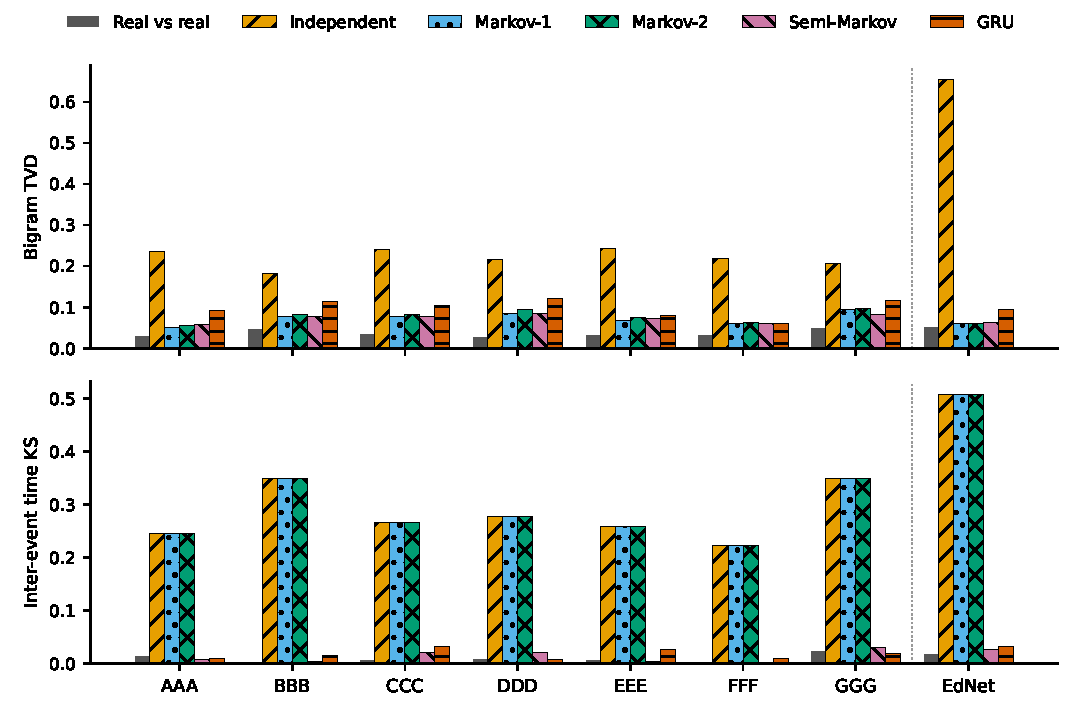
\includegraphics[width=\linewidth]{fig_fidelity.pdf}
\caption{Bigram TVD (top) and inter-event time KS (bottom) per OULAD module
and for EdNet, lower is better. Dark grey: real-versus-real reference;
Markov-1/2: first/second-order Markov; GRU: recurrent neural network.}
\label{fig:fidelity}
\end{figure}

\subsection{Memorisation}
The benchmark's duplication diagnostic compares synthetic data with holdout
learners, which the generator never saw. To test memorisation of
\emph{training} data, we compared synthetic data from the Markov-2,
semi-Markov, and GRU generators with the training learners, using unseen holdout
learners as the baseline (Table~\ref{tab:diagnostics}). Synthetic sessions
reproduced a session seen only once in training about as often as holdout
sessions did (differences of at most 2.3 percentage points, in both
directions); no more synthetic than holdout learners repeated a training
learner's whole sequence of sessions or had a training learner with
identical behavioural features; and median distances to the nearest training
learner were similar or larger. On EdNet, synthetic sessions matched a
training session far less often than holdout sessions (1.8--7.1\% against
20\%; the GRU came closest to the training data), and synthetic learners were
further from the training learners than unseen real learners (median
1.07--1.63 against 0.42): low memorisation, but also a learner-level realism
gap, because sessions are sampled independently of each other. For the same reason these generators cannot reproduce rare
multi-week trajectories. On OULAD, short weekly sessions are common to many
learners (79--88\% of holdout sessions of three or more events also occur
among training learners), so exact duplication alone is not evidence of
memorisation. These diagnostics do not make the output anonymous or safe for
unrestricted sharing.

\begin{table}[t]
\centering
\caption{Stability, memorisation, and detection diagnostics (ranges over
OULAD modules and over the Markov-2, semi-Markov, and GRU generators). ARI: adjusted Rand index
(1~=~identical partitions, 0~=~chance). Memorisation rows compare with the
training learners; ``holdout'' is the baseline of unseen real learners.}
\label{tab:diagnostics}
\resizebox{\linewidth}{!}{\begin{tabular}{l r r }
\toprule
Diagnostic & OULAD (7 modules) & EdNet-KT4 \\
\midrule
Profile stability, seeds (ARI) & 0.93--1.00 & 0.99 \\
Profile stability, 80\% subsamples (ARI) & 0.78--0.95 & 0.98 \\
Profile replication on holdout (ARI) & 0.36--0.84 & 0.93 \\
Profile recovery, synthetic mixture (ARI) & 0.78--0.92 & 0.75 \\
Sessions matching a once-seen training session: holdout & 5.3--8.5\% & 2.8\% \\
\quad synthetic (Markov-2, semi-Markov, GRU) & 5.1--8.9\% & 0.2--1.4\% \\
Learners repeating a training learner's trajectory: holdout & 0.0--3.1\% & 0.0\% \\
\quad synthetic & 0.0--1.4\% & 0.0\% \\
Learners with a feature-identical training learner: holdout & 0.0--8.3\% & 0.0\% \\
\quad synthetic & 0.0--3.7\% & 0.0\% \\
Median distance to nearest training learner: holdout & 0.64--0.90 & 0.42 \\
\quad synthetic & 0.62--0.94 & 1.07--1.63 \\
Detector ROC-AUC: real background & 0.88--0.92 & 0.77 \\
\quad synthetic background & 0.88--0.92 & 0.90 \\
Detector: synthetic vs real normal sessions (AUC) & 0.48--0.52 & 0.49 \\
\bottomrule
\end{tabular}
}
\end{table}

\subsection{Behavioural profiles}
We separate three claims. \emph{Reconstruction}: clustering a synthetic
mixture of the four learned profiles recovered each synthetic learner's
profile (ARI 0.78--0.92 on OULAD, 0.75 on EdNet); this only shows that the
generator preserves its own profiles. \emph{Stability on real data}: on
training learners, assignments agreed across clustering seeds (ARI
0.93--1.00 on OULAD, 0.99 on EdNet) and 80\% subsamples (0.78--0.95; 0.98).
Profiles fitted independently on holdout learners agreed closely on EdNet
(0.93) but only moderately on OULAD (0.36--0.84), where profile boundaries
are therefore not uniquely determined. \emph{Relation to outcomes}
(OULAD, descriptive): without using outcomes, six of seven modules produced a
low-engagement profile whose holdout learners passed in 0--11\% of cases,
against 72--93\% in the most successful profile (NMI 0.10--0.30). Learners
who withdraw stop generating activity, so this partly reflects persistence;
it is neither predictive nor causal evidence, and the profiles are
descriptive clusters, not validated learner types.

\subsection{Detection against ground truth}
Into real holdout sessions we injected two anomaly types, each into a
disjoint random 5\% of sessions: an unexpected transition inserts two events
forming a pair never observed among training learners (labelled invalid
workflow by construction), and a repetition inserts four events alternating
between two of the session's activity types (unusual but valid). Labels are
per session. A simple detector, the mean negative log-likelihood of a
session's transitions under an add-one-smoothed bigram model fitted on
training learners, reached ROC-AUC 0.88--0.92 on OULAD and 0.77 on EdNet
(per-type results in the supplementary material). The detector could not
separate normal synthetic from normal real sessions (AUC 0.48--0.52 and
0.49), so it did not key on generator artefacts. Injecting the same anomalies
into synthetic sessions gave similar ROC-AUC on OULAD but a higher one on
EdNet (0.90 against 0.77): anomalies stood out more against sessions drawn
from a Markov model than against real ones, so synthetic backgrounds can
overstate absolute detector performance and are better suited to comparing
detectors than to estimating their accuracy. Results on real sessions come
from an injection experiment, not from natural anomalies.

\subsection{Cost}
Wall time includes ingestion, sessionisation, and all analyses but not the
one-off conversion of the raw files (37~s for OULAD) or report generation.
On a laptop (Intel Core i9-9880H, 32~GB RAM, one process), the benchmark of
four generators with three seeds took 20--108~s per OULAD module and 59~min
for EdNet, almost all of it in the nearest-neighbour edit distances between
long sessions; the remaining EdNet analyses took 9~min. Training the GRU took
4--47~s per OULAD module and 6~min on EdNet.

%% ---------------------------------------------------------------------------
\section{Impact}

\emph{Demonstrated.} The case studies show that EduLogGen supports, on public
data and with a few commands, a reproducible comparison of generators on
held-out learners against a real-versus-real reference; memorisation
diagnostics against training data; profile stability and recovery analyses;
and known-truth anomaly experiments on both real and synthetic backgrounds.
Each produces numbers that other researchers can regenerate from the
released scripts.

\emph{Potential.} A group that cannot release its logs could publish
synthetic logs together with a validation report, so that others can develop
methods before requesting access to the real data; teachers can give students
realistic logs without personal data; and method developers can study, for
example, how detectors degrade under deadline surges introduced through
controls. Plugins let researchers add readers for other platforms and further
generators, such as larger or tuned neural models, while reusing the
validation and benchmarking machinery.

\emph{Availability.} EduLogGen is installable from PyPI, documented online,
and archived on Zenodo for every release. It was released recently, and no
external adoption is claimed yet.

%% ---------------------------------------------------------------------------
\section{Conclusions}

EduLogGen provides an end-to-end, reproducible workflow for synthetic
educational interaction logs and an experimental layer with known ground
truth. On aggregated weekly activity (OULAD) and on fine-grained clickstreams
(EdNet), its interpretable generators reproduced event frequencies and
session lengths with small discrepancies and improved sequential fidelity
over an order-blind baseline, approaching but not reaching the difference
between two real learner samples; only the semi-Markov and GRU generators
reproduced timing, and the untuned GRU did not improve sequences. Synthetic
data showed no sign of memorising training learners, but
synthetic backgrounds made anomalies easier to detect than real ones did on
EdNet.

The current version has limitations. Markov models capture short-range
dependencies only, the GRU was evaluated without hyperparameter tuning, and
sessions are sampled independently, so long-range
structure such as progression through a course is not reproduced, and
synthetic learners are less realistic as wholes than their sessions are. The
nearest-neighbour diagnostic is slow on long sessions in pure Python. Privacy
diagnostics are empirical and give no formal guarantee such as differential
privacy~\cite{dwork2014dp}. Injected anomalies are synthetic patterns, and
calendar controls have not been validated against observed calendars.
Planned work includes simulated learning outcomes with leakage-safe splits,
scenario files with their own command-line interface, further anomaly types,
and differentially private generators.

%% ---------------------------------------------------------------------------
\section*{CRediT authorship contribution statement}
\textbf{Anis Bey:} Conceptualization, Methodology, Software, Validation,
Formal analysis, Writing -- original draft, Writing -- review \& editing.

\section*{Declaration of competing interest}
The author declares no known competing financial interests or personal
relationships that could have appeared to influence the work reported in
this paper.

\section*{Declaration of generative AI and AI-assisted technologies in the writing process}
During the preparation of this work the author used Claude (Anthropic) to
assist with software development and with drafting parts of this
manuscript. After using this tool, the author reviewed, tested, and edited
the code and the content as needed and takes full responsibility for the
content of the publication.

\section*{Funding}
This research did not receive any specific grant from funding agencies in
the public, commercial, or not-for-profit sectors.

\section*{Data availability}
OULAD~\cite{kuzilek2017oulad} (CC BY 4.0) and EdNet~\cite{choi2020ednet}
(CC BY-NC 4.0) are publicly available. Scripts and aggregate results that
reproduce this study are in the repository (\texttt{studies/}).

\section*{Acknowledgements}
The author thanks the Open University and Riiid for making OULAD and EdNet
publicly available.

\section*{Appendix A. Supplementary material}
Supplementary material (per-module and per-seed results, stability,
memorisation, and per-type detection results) is provided with this article.

\bibliographystyle{elsarticle-num}
\bibliography{references}

\end{document}
